\section{Controlled evidence and prospective evaluation}

\subsection{Registered finite dynamic controls}

We first isolate partial observability without training an encoder.  For each controlled domain,
two hand-selected roots have the same current $32\times32$ rendered frame and different hidden
velocity.  From each root we exhaustively enumerate all $3^3$ sequences on the registered action
grid $\{-1,0,+1\}$ under nominal deterministic dynamics.  Let $V_s(\eta)$ be the full-history
max--min margin-to-go and $Q_s(\eta,a)$ the value after fixing the first action and then allowing
full-history optimal control to resume.  On the viable
members of a code fiber, the first-action obstruction is
\[
 \kappa_s(z)=\min_a\max_{\eta:R_s(\eta)=z,\ V_s(\eta)\geq0}
 [-Q_s(\eta,a)]_+.
\]
Thus $\kappa_s(z)=0$ exactly when the viable histories in that finite fiber share a viable first
action; empty viable fibers use zero.  A separate backward-induction pass constructs a time-indexed
common-safe-action policy and checks retained viability throughout the tree.  Global-policy signs
use exact comparisons on stored binary floats; $10^{-12}$ applies only to numerical-bound checks
and the separately labeled $\kappa_s\leq10^{-12}$ diagnostic.  Here
$h_{\rm cart}=0.82-|p|$ and $h_{\rm pend}=0.70-|\operatorname{wrap}(\theta)|$.

\begin{figure*}[t]
\centering
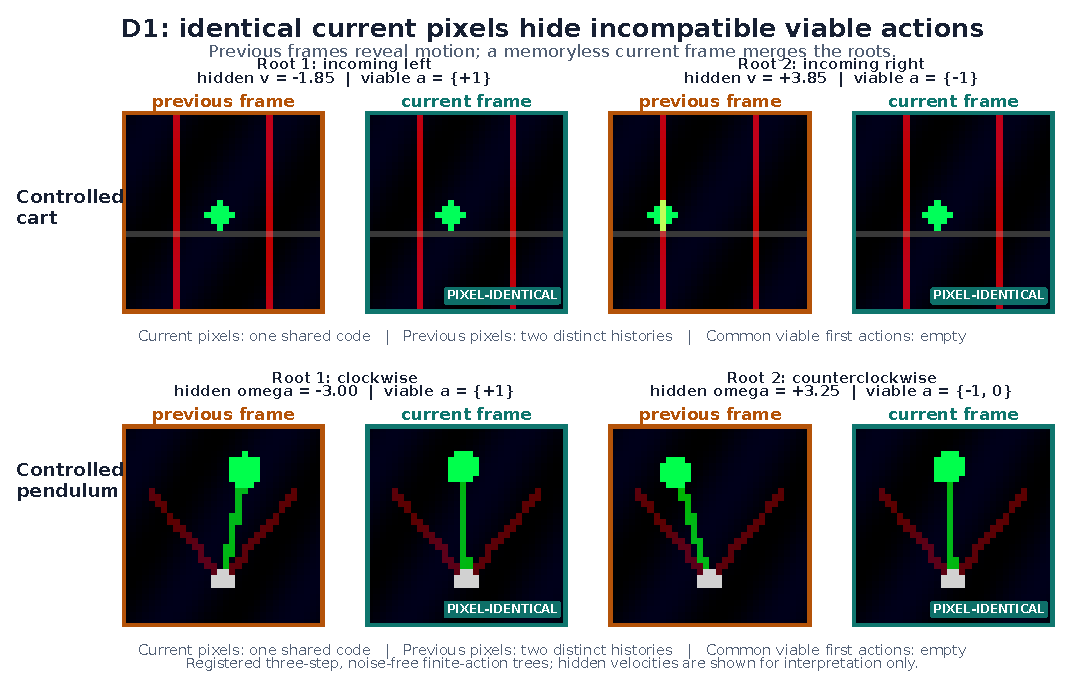
\includegraphics[width=.96\textwidth]{figures/d1_controlled_aliases.pdf}
\caption{Registered D1 hidden-velocity aliases.  Within each domain, the two roots have
pixel-identical current frames but incompatible viable first-action sets; the preceding frame
separates the histories.  Images and action sets are exhaustive only for the declared three-step,
noise-free nominal trees.  Hidden-state labels are explanatory and are not inputs to the
memoryless code.}
\label{fig:d1-controlled-aliases}
\end{figure*}

\begin{table}[H]
\centering
\small
\caption{Exact-code controls on the registered three-step nominal trees.  \emph{Global policy}
means one representation policy preserves every full-history-viable history on all enumerated layers.}
\label{tab:dynamic-controls}
\begin{tabular}{@{}llrc@{}}
\toprule
Domain & representation code & root $\kappa_3$ (native) & global policy \\
\midrule
Cart & privileged state & $0$ & yes \\
Cart & current frame & $0.017987$ & no \\
Cart & causal two-frame history & $0$ & yes \\
Pendulum & privileged state & $0$ & yes \\
Pendulum & current frame & $0.015351$ & no \\
Pendulum & causal two-frame history & $0$ & yes \\
\bottomrule
\end{tabular}
\end{table}

At the cart roots the individually viable action sets are respectively $\{+1\}$ and $\{-1\}$;
at the pendulum roots they are $\{+1\}$ and $\{-1,0\}$.  The exact current-frame code therefore
admits no common viable action in either domain, while the previous frame separates the roots.
Figure~\ref{fig:d1-controlled-aliases} visualizes the registered alias construction, and
Table~\ref{tab:dynamic-controls} reports its exact finite-tree audit.  Both are provisionally
internally verified finite floating-point
fixtures, not learned-model or population evidence; their scope is the declared roots, actions,
horizon, arithmetic semantics, and noise-free model.  The
cart roots also lie outside the behavior generator's nominal velocity envelope.  Exact roots,
configuration, and the producing command are registered under D1-controlled-dynamic-oracle in the
repository claim ledger.

\subsection{Prospective pretrained-representation study}
\label{sec:prospective-study}

No pretrained-encoder result is reported.  The checked-in AE/$\beta$-VAE cart, pendulum, and Dubins
pipeline remains an engineering precursor for estimator, profile-label, and confirmatory-analysis
plumbing; it is not the headline empirical study and supplies no foundation-model evidence.  The
new protocol addresses three questions: whether standard pretrained features exhibit safe-choice
aliasing, whether the proposed audit predicts closed-loop failures beyond native utility and a
safety probe, and whether an internal encoder repair improves both quantities without erasing the
original representation utility.

\paragraph{Pretrained families and information matching.}
The primary frozen checkpoints deliberately span three objectives.  Cosmos Tokenizer supplies
continuous and discrete causal video codes at controlled spatial and temporal compression rates
\citep{nvidia2025cosmos,nvidia2025cosmostokenizer}.  V-JEPA~2.1 ViT-B supplies dense temporal
predictive features, with V-JEPA~2-AC as an action-conditioned sensitivity
\citep{assran2025vjepa2,murlabadia2026vjepa21}.  DINOv3 ViT-S/B supplies semantic and dense spatial
features \citep{simeoni2025dinov3}.  Every model receives the same causal RGB clip, time span, and
available proprioceptive variables.  Because DINO is image-based, its patch features are encoded
framewise and passed through the same capacity-matched temporal aggregator used in the standardized
comparison.  We report both each model's native interface and a matched-rate interface with the
same token/bit budget and downstream pooling capacity; full token grids and pooled decision states
are audited separately.  Continuous features use a registered quantizer and numerical precision;
floating-point dimension alone is not treated as bitrate.  Cross-family results are descriptive
because architecture, scale, and pretraining data differ.  A smaller matched-backbone, matched-data
objective ablation is required
before attributing differences causally to the pretraining objective.

\paragraph{Two primary physical domains.}
The first target is contact-rich manipulation in ManiSkill3
\citep{tao2025maniskill3}.  A finite library contains short Cartesian end-effector motions and
gripper skills; profiles record minimum collision-clearance, joint-limit, contact-force, workspace,
and object-drop margins.  The second target is embodied navigation in Habitat
\citep{savva2019habitat}.  Its library contains short velocity or waypoint skills; profiles record
minimum obstacle clearance, stopping margin, and, when present, distance to moving agents.  The two
domains differ in appearance, dynamics, contact, and action semantics.  Driving may be added as a
third external-validity study, but no driving-specific model is required for the core claim.

Each example begins from a saved simulator state.  The encoder receives observations only, while
the data generator branches that state under every registered skill to produce $q_H(x,\cdot)$.
This privileged counterfactual oracle is the primary mechanism experiment, not a deployment claim.
A cross-fitted action-conditioned teacher trained without held-out simulator state is a realism
ablation and must report profile error and abstain near the safety boundary.  Raw causal video and
privileged physical state provide information upper bounds; one-frame observations and exact aliases
isolate the observation floor.

\paragraph{Repair and baseline arms.}
Within each pretrained family, data, history, trainable parameter count, optimizer steps, and
readout capacity are paired.  The required arms are: frozen encoder plus profile head; native-loss-
only internal adaptation; scalar-margin and frozen FCSRL-style feasibility adaptation
\citep{cen2024feasibility}; internal profile-only adaptation; pairwise conflict separation; the full
set-wise repair; and a post-code adapter explicitly labeled geometry-only.  Shuffled profiles,
conflict-count-matched random groups, true-profile append, and full fine-tuning are controls.  The
same profile head is removed from every learned arm before a fresh head and controller are trained.
Recent planning-aware driving tokenization already supplements reconstruction with representation
and geometry signals \citep{yao2026unified}; accordingly, a generic auxiliary-loss improvement is
not the claimed contribution.

\paragraph{Endpoints and held-fixed downstream test.}
The primary representation endpoint is the trajectory-balanced tail of $v_i(\delta)$, normalized by
physical margin scale and reported as a frozen radius curve, at matched neighborhood mass or fixed
$k$, and on physically generated groups.  Coverage, duplicate rate, effective rank, distance
distortion, and token entropy accompany every value.  Family-specific native utility is assessed
against its own frozen checkpoint---reconstruction/perceptual/rate metrics for Cosmos, latent
prediction for V-JEPA, and frozen dense-feature transfer for DINO---and is not averaged across
families.

For downstream evaluation, one frozen nominal controller proposes or ranks the same registered
skills in each condition.  A freshly trained capacity-matched safety readout filters or reranks
them, after which controller parameters remain fixed.  Primary outcomes are constraint violations
and near misses; task success, return, intervention rate, and control effort are joint utility
outcomes.  We test whether the common-action audit adds leave-one-domain-out predictive value beyond
native utility, ordinary action prediction, and scalar-safety probe metrics.  Appearance shifts,
unseen hazard mechanisms, safety thresholds, profile horizons, and denser action libraries test
specification and distribution transfer.

\paragraph{Advancement and falsification gates.}
All repair comparisons use fresh paired seeds and a validation-frozen utility noninferiority margin
before test access.  The foundation study advances only if raw causal observations predict the
registered profiles, the defect survives information/rate matching in both domains and at least two
families, the full internal repair beats an identical frozen-head and native-adapter control, and
the improvement survives head removal, matched-neighborhood-mass auditing, and a fresh downstream
controller.  The thesis is rejected or narrowed if observation ambiguity explains the effect, a
head-only model matches repair, representation gains come only from norm expansion or empty
neighborhoods, scalar feasibility dominates, or the audit adds no information about closed-loop
violations.
